\documentclass[oneside,openright,frontopenright]{dmathesis}
\usepackage[utf8]{inputenc}
\usepackage[T1]{fontenc}
\usepackage{lmodern}
\usepackage[british]{babel}
\usepackage[figuresright]{rotating}
\usepackage[draft=false,protrusion=true,expansion,shrink=10,stretch=10,]{microtype}
\makeatletter
\@ifpackageloaded{microtype}{%
	\providecommand{\disableprotrusion}{\microtypesetup{protrusion=false}}
	\providecommand{\enableprotrusion}{\microtypesetup{protrusion=true}}
}{%
	\providecommand{\disableprotrusion}{}
	\providecommand{\enableprotrusion}{}
}
\makeatother

\usepackage{csquotes}


\usepackage{amsmath,amsthm,amssymb}
\usepackage[hidelinks,draft=false]{hyperref}
\usepackage{booktabs}
\usepackage{xfrac}

% The folder in which images are stored for this project.
% If this is enabled, the folder doesn't need to be specified in each
% call to \includegraphics, i.e
%   \includegraphics{picturename}
% rather than
%   \includegraphics{img/picturename}
%\graphicspath{./img}

% Thmtools sets up theorem-like environments, and modifies the autoref
% command from hyperref to work when these environments share a counter
% Thmtools also defines an Autoref command for capitalising at the start
% of a sentence
\usepackage{thmtools}
\declaretheorem[
style=plain,
name=Theorem,
numberwithin=section
]{thm}
\declaretheorem[
style=plain,
name=Proposition,
numberlike=thm
]{prop}
\declaretheorem[
style=plain,
name=Lemma,
numberlike=thm
]{lem}
\declaretheorem[
style=plain,
name=Corollary,
numberlike=thm
]{cor}
\declaretheorem[
style=definition,
name=Definition,
numberlike=thm
]{mdef}
\declaretheorem[
style=definition,
name=Example,
numberlike=thm
]{example}
\declaretheorem[
style=definition,
name=Remark,
numberlike=thm
]{rem}
\declaretheorem[
style=plain,
name=Conjecture,
numberlike=thm
]{conj}
\declaretheorem[
style=plain,
name=Question,
numberlike=thm
]{question}

\numberwithin{equation}{section}
\allowdisplaybreaks

% Makes the last line of a page flush wtih the bottom margin for neatness
%\raggedbottom
%\emergencystretch=1em
\flushbottom

% use these to make paragraphs not indented,
% and to separate consecutive paragraphs
\setlength{\parindent}{0pt}
\setlength{\parskip}{0.5em plus 3pt minus 3pt}

% Provide itemize without extra spacing
\newenvironment{itemize*}%
{\begin{itemize}%
	\setlength{\itemsep}{0pt}%
	\setlength{\parskip}{0pt}}%
{\end{itemize}}
\newenvironment{enumerate*}%
{\begin{enumerate}%
	\setlength{\itemsep}{0pt}%
	\setlength{\parskip}{0pt}}%
{\end{enumerate}}

% Format captions
\usepackage[margin=15mm,hang]{caption}
\usepackage{subcaption}

\setfloatlocations{figure}{tbp}
\setfloatlocations{table}{tbp}

% In align*, use this to number a particular line
% Rather than using align, and \nonumber-ing every other line
\newcommand\numberthis{\addtocounter{equation}{1}\tag{\theequation}}
% Change autoref names. Generally I want sections to be capitalised at all
% times, not just when starting a sentence.
% (I'm not sure whether all these are necessary nor what the defaults are)
\renewcommand{\equationautorefname}{equation}
\newcommand{\equationAutorefname}{Equation}
\newcommand{\sectionAutorefname}{Section}
\newcommand{\chapterAutorefname}{Chapter}
\newcommand{\subsectionAutorefname}{Subsection}
\newcommand{\subsubsectionAutorefname}{Subsection}
\newcommand{\algorithmAutorefname}{Algorithm}
% Annoyingly these defs need to come *after* \begin{document}, so add to begin
% document hook.
\AtBeginDocument{%
	\def\sectionautorefname{Section}%
	\def\chapterautorefname{Chapter}%
	\def\subsectionautorefname{Subsection}%
	\def\subsubsectionautorefname{Subsection}%
	\def\algorithmautorefname{Algorithm}%
}
\usepackage{cite}
\begin{document}
\title{Null geodesics}
\subtitle{Modelling light in the Schwartzschild metric}
\author{Joseph A Sweeney}
\researchgroup{Mathematics}
\pagenumbering{roman}
\maketitlepage*

\begin{abstract}
%
	In this paper I will show and discuss my findings on numerical methods and optimisations for modelling solutions to the equations of motion deried from geodesic equations in the Schwarzschild and Kerr metric using Python. In the first section, I will introduce some key information and language associated with General Relativity, which this paper will rely upon. Then, I will demonstrate methods for modelling null (light-like) geodesics about a metric. Using these I will model various black holes as seen directly in front of an observer with any given celestial sphere.
%
\end{abstract}

\begin{declaration*}
%
	The work in this thesis is based on research carried out in the Department of
	Mathematical Sciences at Durham University. No part of this thesis has been
	submitted elsewhere for any degree or qualification.
%
\end{declaration*}

\disableprotrusion
\tableofcontents*
\enableprotrusion

\cleardoublepage
\pagenumbering{arabic}

%\include{background}
%\include{paper1}
%\include{paper2}
%\include{paper3}
\begin{introduction}

	The field of black hole imaging in Physics and Computer Science had a wave of enthusiasm 
	and development following Christopher Nolan’s 2014 blockbuster Interstellar\cite{Interstellar}, and the imaging of the supermassive 
	black hole at the centre of M87 by the Event Horizon Telescope in 2019\cite{event2019first}. Producing high quality images 
	and videos of black holes and wormholes can be very computationally costly, so ingenious ways of gaining 
	efficacy must often be used. My aim is to explore these methods and tricks to present practical approaches 
	to modelling the Schwarzschild metric and Kerr metric. After this I will explore accretion discs and gravitational redshift to create as realistic a model as possible.

\end{introduction}

\chapter{Introduction to General Relativity}
	Albert Einstein’s theory of General Relativity is a pivotal achievement in the scientific community, here, I will attempt to briefly summarise some key components and notation for ease of readers in later sections.

	In his theory of General Relativity, Einstein formalised gravity not as a force - as it is thought of in Newtonian physics - but as the curvature of spacetime. Spacetime is the 4-dimentional plane we exist in, one dimension representing time, and three space. The path of an object acted upon solely by gravity can be thought of as moving along curved spacetime, with the path being a straight line if the effects of gravity are non-existent. Such a path through curved spacetime is called a geodesic, and equations of motion in General Relativity are governed by constants derived from geodesic equations – which in turn are derived from the metric in which the object finds itself. A null-geodesic, or light-like geodesic, is a path describing the motion of a massless object: In this paper, a null-geodesic will always be describing the path of a light particle in a metric. Geodesic equations can be thought of as a generalisation of Newton's second law of motion, taking into account the curvature of the spacetime one chooses. I.e instead of F = 0 $\Rightarrow$ a = 0, we have that F = 0 implies that acceleration is sufficient to keep the motion in a straight line when considered in ordinary space.

	As is common in papers studying light and the astrological, I will be using natural units: That is, I will be taking c = G = 1, this results in non-SI units, but conversion is possible and generally simple. A distance of 1 will correspond to $1$(s) x c($ms^{-1}$) = the distance travelled by light in a vaccum in one second.

	The celestial sphere from a point in space is an image of all the points taken to be arbitrarily far away - for earth it is the sky in all directions excluding the moon, mercury and mars. (My 'arbitrary distance' is t=1000 i.e the distance light travels in a vaccum in 1000 seconds)

	Metrics are sections of spacetime which are solutions to Einstein’s field equations, the equations that define his General theory. As an example, the simplest solution to these field equations describing a black hole is the Schwarzschild metric. A metric is generally given in line notation - which informs one how a change in space relates to changes in the variables we consider the object to be moving in. The relation between geodesic equations and metrics are governed by Christoffel symbols, denoted $\Gamma$, seen in the below general form of a geodesic equation\cite{geodesic}:  


	\[\frac{d^2 \gamma^\lambda}{dt^2} + {\Gamma^\lambda}_{\mu\nu} \frac{d\gamma^\mu}{dt} \frac{d\gamma^\nu}{dt} = 0\]

	Christoffel symbols are incredibly important in the study of General Relativity, relating directly to the Riemann tensor, Metric tensor and other key concepts. Below I will give a sense as to what they represent, but will not dive any further, standing on the shoulders of giants by relying on equations derived and examined over many years.

	The Christoffel symbols are related to the coefficients in the line metric, and can be quite messy as they consider all relations between variables. Below is the general form of the Christoffel symbol using Einsteins summation convention\cite{albert1916foundation}:
	
	\[{\Gamma^\lambda}_{\mu\nu} = \frac{1}{2}g^{\lambda{l}}(\partial_{\nu}g_{\mu{l}} + \partial_{\mu}g_{l\nu} + \partial_{l}g_{\mu\nu})\]
	
	Here, g is the matrix of coefficients in the metric - g is also confusingly called the metric but this is as it determines the line notation completely. $g_{ij}$ is the (i,j)'th component of g, and $g^{ij} = {g^{-1}}_{ij}$ is the (i,j)th component of the inverse of g.

\chapter{Solving general relativistic equations of motion}
\section{Deriving the equations of motion}
	Equipped with the equations of motion derived from the geodesic equation determined by the metric we are given; we can visualise the path of light in such a metric by solving these equations numerically. We will start with the Schwarzschild metric, given in line notation by\cite{derivationSchwarzschild}: 


	\[{ds^{2} = {\left(1-\frac {2m}{r}\right)}^{-1}} {dr^2} + {r^2}({d\theta ^2} + {\mbox{sin} ^2}{\theta}{d\varphi ^2}) -{\left(1-\frac {2m}{r}\right)}{dt^2}\]


	Since the metric is spherically symmetric, we see that every path will always be contained in a plane intersecting the origin of the black hole. Therefore, without loss of generality we can take ${\theta}=\frac{\pi}{2}$ and observe from 'above’ the equatorial plane to see the path of such a light ray in the plane.

	From the above equation, one can derive the equations of motion of a null geodesic in the Schwarzschild metric:


	\[\ddot{r}=-\frac{L^2(3M-r)}{r^4}\]

	\[\dot{\varphi}=\frac{L}{r^2}\]


	Where M is the mass of the black hole, L is a constant proportional to the angular momentum of the light ray, r is the distance from the centre of the black hole, and $\varphi$ is the angle from the positive x axis to the light ray.

\section{Method for solving the system}
	The simplest method of solving such an equation numerically is to split the equation into a coupled first order differential equation. Then use a numerical approximation to update r, $\dot{r}$ and $\varphi$ for each point in a time array, if you keep track of r and $\varphi$ for all points in the time array you can then plot the path. One thing to be careful about is that as soon as light is within r = 2M, solutions will not make any sense, so we cannot have an initial position in this region, and ideally while keeping track of r, cut the process off when r = 2M.

	This method is both the simplest and most effective for solving second order ODE’s numerically, the only difference between a ‘bad’ and ‘good’ method would be the choice of numerical approximation method to solve the first order ODE’s.

	Below are the coupled differential equations equivalent to the equations of motion:

	\[\dot{r}= s\]

	\[\dot{s}=-\frac{L^2(3M-r)}{r^4}\]

	\[\dot{\varphi}=\frac{L}{r^2}\]

\begin{figure}
	\centering
	\begin{minipage}[b]{0.6\textwidth}
		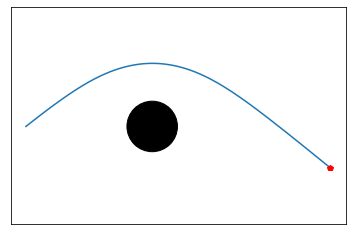
\includegraphics[width=\textwidth]{img/points200byhand}
		\caption{A plot with 200 points in the time array using short distances in Cartesian coordinates to approximate the slope of the line and continue in that direction}
	\end{minipage}
	\hfill
	\begin{minipage}[b]{0.6\textwidth}
		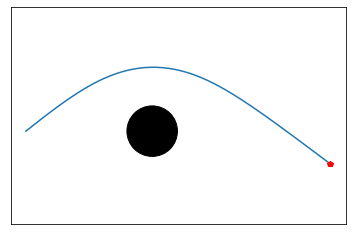
\includegraphics[width=\textwidth]{img/points200scipy}
		\caption{A plot with 200 points in the time array using scipy.integrate.solve\_ivp}
	\end{minipage}
\end{figure}


	I have found that for a plot of the path of a photon (Figure 1), the ideal method is solve\_ivp\cite{2020SciPy-NMeth}, using LSODA\cite{hindmarsh2005lsoda}, this is as the Explicit Runge-Kutta method of order 5 (RK45)\cite{fehlberg1969low}, the inherent method used by solve\_ivp is very efficient but not smooth, so makes for unattractive plots. Later, when a plot is not required, I will be using RK45. Also, solve\_ivp allows one to keep track of an ‘event’, and return if the event took place, moreover one may choose to cut off the calculation process when such an event takes place. Naturally this is very useful in our case, as all we need to set the event to is r < 2M.


\chapter{Imaging a Schwarzschild black hole}
\section{Outline of the method}

	We now have the means to start thinking about how to model a black hole of distance r away from a camera, with any given celestial sphere.

	Firstly, we would like to find an equation linking alpha and L, as this would allow us to choose a launch angle and calculate the required parameters for such an angle.

	Then, for modelling a Schwarzschild black hole will be to first find the minimum angle one may fire a photon from the camera without the photon being absorbed by the singularity. For all angles between this minimum angle and just under $\frac{\pi}{2}$ (for this value I take 1.55), we will find a relation between angle fired and final angle after t=1000. The reason we do not go up to $\frac{\pi}{2}$ itself is because as seen later we take tan($\alpha$), which of course is undefined at $\alpha = \frac{\pi}{2}$. By taking L to be very large we can see where the reasonable limit for us to calculate lies - this happens to be approximately 1.55.

	We will then conceptualise a pinhole camera, with its focal point distance r from the centre of the black hole the position of our camera which fires light rays. Using the relation outlined above, we can take any given line straight of pixels which passes through the centre of the image we take as our celesial sphere, and see where each pixel should end up. Then, by 'rotating' the pinhole camera - or by rotating this central line, we may find where each pixel in our new picture draws its light from on the celestial sphere.

\section{How to aquire the launch angle}

	For the rest of this paper we refer to a given photon's launch angle by $\alpha$. We would like to use the equations of motion at t = 0 to discover what value of L with given $\dot{r}$(0) leads to a specific $\alpha$.

	As we are in polar coordinates, 

			\[(x, y) = (r\mbox{cos}(\varphi), r\mbox{sin}(\phi)) \Rightarrow (\dot{x}, \dot{y}) = (\dot{r}\mbox{cos}(\varphi) - r\dot{\varphi}\mbox{sin}(\varphi), \dot{r}\mbox{sin}(\varphi) + r\dot{\varphi}\mbox{cos}(\varphi))\]
	
	Via basic geometry we see that 
			
			\[\mbox{tan}(\alpha) = \frac{\dot{y}(0)}{\dot{x}(0)} = \frac{\dot{r}(0)\mbox{sin}(\varphi(0)) + r(0)\dot{\varphi}(0)\mbox{cos}(\varphi(0)}{\dot{r}(0)\mbox{cos}(\varphi(0)) - r(0)\dot{\varphi}(0)\mbox{sin}(\varphi(0))}\]

	So we obtain that 

			\[ L = \frac{r(0)\dot{r}(0)(\mbox{cos}(\varphi(0))\mbox{tan}(\alpha)-\mbox{sin}(\varphi(0))}{\mbox{cos}(\varphi(0))+\mbox{sin}(\varphi(0))\mbox{tan}(\alpha)}\]

\section{Finding $\alpha_{min}$}
	
	To find the minimum angle at which a light ray escapes the gravitational pull of the black hole, I send out a number of angles ranging from 0 to $\frac{\pi}{2}$, then, as soon as an angle does not lead to a termination of solve\_ivp, I repeat this process with much smaller intervals between the previous and current angle. This leads to an accurate $\alpha_{min}$.

\section{The relationship between $\alpha$ and $\alpha^{'}$}

	By running this program across angles from $\alpha_{min}$ to 1.55 and plotting $\alpha$ on the x-axis with $\alpha^{'}$ on the y axis we find the relationship between $\alpha$ and $\alpha^{'}$. For $\alpha$ between -1.55 and -$\alpha_{min}$ we may take -f(-$\alpha$), where f is the function relating the two. Here we have covered -1.55 to 1.55 radii, more than a full field of view.

	Here,  $\alpha^{'}$ is the angle from the camera to the final position of the light ray (See Figure 3.2).

	When $\alpha \approx \alpha_{min}$ or $-\alpha \approx -\alpha_{min}$ the light ray might semi-orbit or even fully orbit the black hole, meaning I had to be careful in my method  of calculating $\alpha^{'}$. To avoid errors I kept track of the change in $\varphi$, the angle from the current position of the ray to the centre of the black hole. When taking this value modulo $2\pi$, I could see how many orbits the ray had undergone. The main issue with not doing this is for a plot of the function 4, in application we want the angle $-\pi<\alpha^{'}<\pi$.

\begin{figure}
	\centering
	\begin{minipage}[b]{0.6\textwidth}
		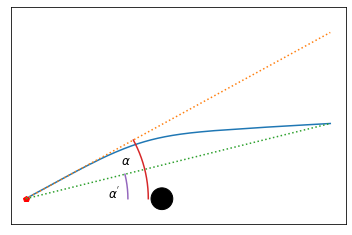
\includegraphics[width=\textwidth]{img/alpha_alpha-prime}
		\caption{A plot with $\alpha$ = 0.5, $\alpha^{'}$ = 0.242 at an initial distance of 100 along the equatorial plane (t = [0,200], r(0) = 100, $\dot{r}$(0) = -1, $\varphi$(0) = -$\pi$, M = 4)}
	\end{minipage}
	\hfill
	\begin{minipage}[b]{0.6\textwidth}
		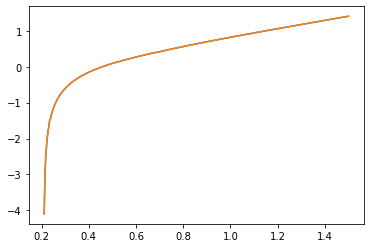
\includegraphics[width=\textwidth]{img/alpha-prime_f(alpha)}
		\caption{A plot of the function f, relating $\alpha$ to $\alpha^{'}$ (t = [0,1000], r(0) = 100, $\dot{r}$(0) = -1, $\varphi$(0) = -$\pi$, M = 4)}
	\end{minipage}
\end{figure}

\section{Modelling the black hole}
	
	As outlined in 3.1, here we will give our code a star field to treat as a celestial sphere, and see how a black hole affects the image. To do this, the first thing we do is to calculate the distance in pixels from the middle of the picture to a corner, this will be our 1.55 radians. Then, for every pixel on the original image we calculate the angle $\alpha$ implied by the distance from the pixel to the centre of the image. Then, we use an interpolation technique on our relationship between $\alpha$ and $\alpha^{'}$ to calculate the angle along the straight line intersecting the current pixel and the central pixel at which the light ray would end. Then by converting this angle back to distance we update a copy of the picture to switch the current pixel for the closest pixel to the end point on the original picture.

\begin{figure}
	\centering
	\begin{minipage}[b]{0.6\textwidth}
		\includegraphics[width=\textwidth]{img/8kstarfield-special}
		\caption{A model highlighting areas affected by the limited size of the image}
	\end{minipage}
\hfill
	\begin{minipage}[b]{0.6\textwidth}
		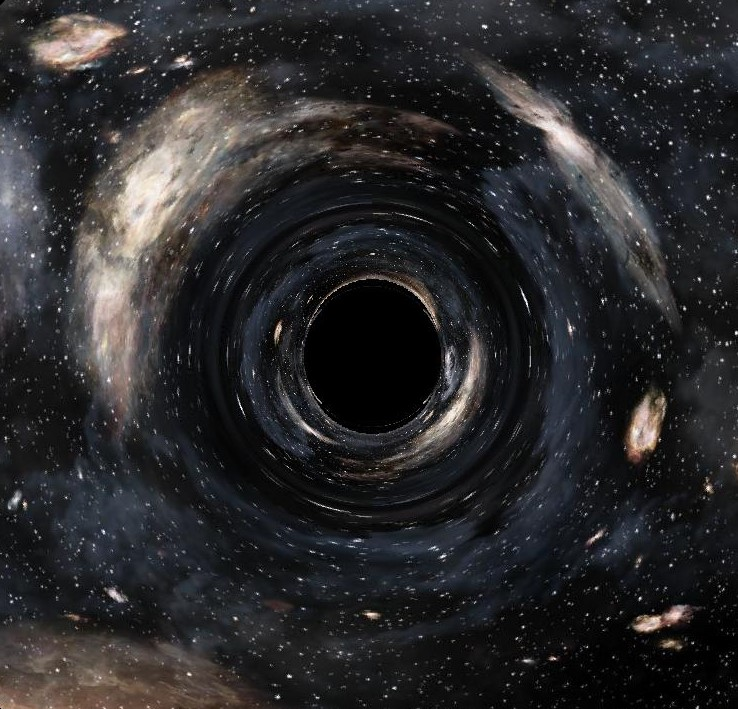
\includegraphics[width=\textwidth]{img/hdri-pov}
		\caption{A model using a HDRI image for the celestial sphere, mapped back to ordinary coordinates and cropped to show POV. Credit for original image: Double Negative \url{https://www.dneg.com/interstellar-wormhole}}
	\end{minipage}
\end{figure}

	One issue that I had when first modelling these black holes is that I was not using an image covering $4\pi$ steradians, meaning any ray which leaves the area covered by the original image would lead to a black pixel. This leads to an irregularly shaped black hole (See Figure 3.4), if the image I used as a celestial sphere were circular, the black hole would seemingly look ordinary, as the irregularities would be smoothed out horizontally and vertically, but would be too large. My solution to this was to use a HDRI image as my celesial sphere and crop for a reasonable field of view (See figure 3.5).


\chapter{Kerr black holes}
\section{Properties of black holes}

	In this section I will move on to more general black holes, specifically ones with non-zero spin, I will introduce the Kerr metric and take a look at the equations of motions derived from the geodesic equation of light in the Kerr metric.

	Black holes are simultaniously one of the simplest and complicated objects known to exist in the universe: On the one hand, we can only theorise what happens as black holes age, or what happens beyond the event horizon - but on the other, black holes are defined entriely by only three properties. This is extraordinary, especially when considering their size and significance.

	The three properties which define a black hole are mass, spin, and charge. Any two black holes with all three properties the same are essentially equivalent. Different metrics are given for describing black holes, these are usually to simplify things taking either spin or charge to be zero. For example the Schwarschild metric, which we have been working with, is the simplest such metric - taking both spin and charge to be zero. The Kerr metric takes only charge to be zero, and spin affects the curvature of spacetime rather substantially. A charged, non-spinning black hole is described by the Reissner–Nordström metric, and finally, the most general metric describing a black hole is the Kerr-Newman metric - taking mass, spin and charge to all be non-zero. Of course one could use the equations of motion implied by the hamiltonian of the geodesic equation generated by the Kerr-Newman metric and take spin and/or charge to be zero rather than using other metrics - but this requires much more work.

\section{The Kerr metric}

	The Kerr metric of a mass M rotating with angular momentum per unit mass a = $\frac{J}{M}$ is given by \cite{raquepas2017topics}:

	\[{ds^{2} = -\frac{\Delta}{\Sigma}(dt-a\mbox{sin}^2(\theta)d\varphi)^2+\frac{\mbox{sin}^2(\theta)}{\Sigma}((r^2+a^2)d\varphi-adt)^2)+\frac{\Sigma}{\Delta}dr^2+\Sigma d\theta^2}\]

	With:
	
	\[\Delta(r) := r^2 - 2Mr + a^2\]
	\[\Sigma(r, \theta) := r^2 +(a\mbox{cos}(\theta))^2\]

	This is using what is called Boyer-Lindquist coordinates, which are similar to spherical polar coordinates but 'stretched'. They are related to real Euclidean space by:

	\[t=t\]
	\[x = \sqrt{r^2+a^2}\mbox{sin}(\theta)\mbox{cos}(\varphi)\]
	\[y = \sqrt{r^2+a^2}\mbox{sin}(\theta)\mbox{sin}(\varphi)\]
	\[z = rcos(\theta)\]

	Using the Hamiltonian formalisation and via Noether's theorem and Hamilton-Jacobi theorem we find four constants of motion from the geodesic equation \cite{}:

	\[\mu = \mbox{mass of particle} = 0\mbox{ for us}\]
	\[E = -p_t\]
	\[L_z = p_{\varphi}\]
	\[Q = {p_{\theta}}^2+\mbox{cos}^2(\theta)\left(a^2(\mu^2-E^2)+\left(\frac{L_z}{\mbox{sin}(\theta)}\right)^2\right)\]

	Then using these constants we can write the equations of motion as:

	\[\dot{r} = \pm\frac{\sqrt{R(r)}}{\Sigma}\]
	\[\dot{\theta} = \pm\frac{\Theta(\theta)}{\Sigma}\]
	\[\dot{\varphi} = \frac{1}{\Sigma}\left(\frac{L_z}{\mbox{sin}^2(\theta)}-aE+\frac{a}{\Delta}P(r)\right)\]
	\[\dot{t} = \frac{1}{\Sigma}\left(-a(aEsin^2(\theta)-L_z)+\frac{r^2+a^2}{\Delta}P(r)\right)\]

	With:

	\[\Theta(\theta) = Q - \mbox{cos}^2(\theta)\left(\frac{{L_z}^2}{\mbox{sin}^2(\theta)}-a^2E^2\right)\]
	\[P(r) = E(r^2+a^2)-aL_z\]
	\[R(r) = P(r)^2-\Delta\left((L_z-aE)^2+Q)\right)\]

\appendix
%\include{appendix1}
%\include{appendix2}

%\nocite{}
\bibliographystyle{plain}
\bibliography{bibliography}{}
\end{document}